\section*{Folgen}

$\displaystyle\lim_{n \to \infty} = a \Leftrightarrow \forall \epsilon > 0 \exists N_\epsilon \in \N \forall n \geq N_\epsilon : | a_n - a | \leq \epsilon$

\subsection*{Konvergenzsatz für monotone Folgen}

Sei $(a_n)$ wachsend und nach oben beschränkt \\ $\Rightarrow \exists \lim_{n \to \infty} a_n = \sup_{n\geq 1} a_n := \sup\{a_n | n \in \N\}$

Analoges für fallende, nach unten beschr. Folgen.

\subsection*{Bolzano-Weierstraß}

Jede beschränkte Folge hat einen Häufungspunkt

$\overline\lim_{x \to \infty} a_n$ Maximum der Häufungspunkte

$\underline\lim_{x \to \infty} a_n$ Minimum der Häufungspunkte

\subsection*{Cauchyfolgen}

$\forall \epsilon > 0 \exists N_\epsilon \in \N \forall n, m \geq N_\epsilon : | a_n - a_m | \leq \epsilon$

Cauchyfolge $\Leftrightarrow$ konvergente Folge

\subsection*{Uneigentliche Grenzwerte}

Sei $\overline{\R} = \R \cup \{-\infty, +\infty\}$

$\forall K \in \N \exists N_K \in \N \forall n \geq N_K : x_n \geq K \Leftrightarrow \displaystyle\lim_{n \to \infty} x_n = \infty$

\subsection*{Beispiele und Hinweise}

\[ e^x = exp(x) = \lim_{n\to \infty} \Big(1 + \frac{x}{n}\Big)^n \text{ insb. } e = \lim_{n\to \infty} \Big(1 + \frac{1}{n}\Big)^n \]

Zur Bestimmung von Folgen Grenzwerten kann auch L'Hospital herangezogen werden.

\section*{Reihen}

Sei $(a_k)_{k\geq 0}$ Folge, dann ist $\sum_{k\geq 0} a_k$ Reihe.

\subsection*{Konvergenzkriterien}

$\sum_{k=0}^\infty a_k = \lim_{n\to \infty} \sum_{k=0}^n a_k = \lim_{n\to \infty} s_n$

$\sum_{k\geq 0} a_k$ konvergiert $\Rightarrow (a_k)$ ist Nullfolge.

\subsubsection*{Leibnizkriterium}

Es gelte $\forall k \in \N_0 : b_k \geq b_{k+1} \geq 0$ und $\displaystyle \lim_{k \to \infty} b_k = 0$

Dann konvergiert: $\sum_{k=0}^\infty (-1)^k b_k$

\subsubsection*{Majorantenkriterium}

\begin{enumerate}[label=(\alph*)]
	\item Wenn $0 \leq |a_k| \leq b_k \forall k \in \N_0$ und $\sum_k b_k$ konvergiert, dann konvergiert $\sum_k a_k$ absolut und es gilt $|\sum_{k=0}^\infty a_k| \leq \sum_{k=0}^\infty |a_k| \leq \sum_{k=0}^\infty b_k$.
	\item Wenn $a_k \geq b_k \geq 0$ und $\sum_k b_k$ divergiert, dann divergiert $\sum_k a_k$
\end{enumerate}

\subsubsection*{Quotientenkriterium}

Sei $(a_n)_{n\geq 0}$ Folge, $n_0 \in \N$ mit $\forall n \geq n_0 : a_n \neq 0$

$\overline\lim_{n \to \infty} |\frac{a_{n+1}}{a_n}| < 1 \implies \sum a_n$ konvergiert absolut

$\underline\lim_{n \to \infty} |\frac{a_{n+1}}{a_n}| > 1 \implies \sum_{n\geq 0} a_n$ divergiert

\subsubsection*{Wurzelkriterium}

\vspace*{-4mm}
\begin{align*}
	\overline\lim_{n \to \infty} \sqrt[n]{|a_n|} < 1 &\implies \textstyle\sum_{n\geq 1} a_n \text{ konvergiert} \\
	\overline\lim_{n \to \infty} \sqrt[n]{|a_n|} > 1 &\implies \textstyle\sum_{n\geq 1} a_n \text{ divergiert} \\
	(b_n) \text{ unbeschränkt } &\implies \textstyle\sum_{n\geq 0} a_n \text{ divergiert}
\end{align*}

\subsubsection*{Integralkriterium}

Für monoton fallende Koeffizientenfolge $f$ gilt:

$\int_p^\infty f(n) dn$ integrierbar $\Leftrightarrow \sum_{n=p}^\infty f(n)$ konvergiert.

\subsection*{Beispiele}

\vspace*{-8mm}
\begin{align*}
	\textstyle\sum_{n=0}^\infty \frac{x^n}{n!} &= e^x \text{ (insb. } \textstyle\sum_{k=0}^{\infty} \frac{1}{k!} = e) \\
	\textstyle\sum_{k=0}^{\infty} z^k &= \frac{1}{1-z} (z \in \mathbb{C} \land |z|<1) \\
	\textstyle\sum_{k=0}^{\infty} (\alpha a_k + \beta b_k) &= \alpha \textstyle\sum_{k=0}^{\infty} a_k + \beta \textstyle\sum_{k=0}^{\infty} b_k
\end{align*}
\vspace*{-4mm}

Die allgemeine harmonische Reihe $\sum_{k=0}^\infty \frac{1}{k^\alpha}$ divergiert für $\alpha \leq 1$ und konvergiert für $\alpha > 1$.

\subsection*{Cauchykriterium}

Eine Reihe $\sum_k a_k$ konvergiert genau dann, wenn:

$\forall \epsilon > 0 \exists N_\epsilon \in \N \forall n > m \geq N_\epsilon : | \sum_{k=m+1}^{n} a_k | \leq \epsilon$

\section*{Potenzreihen}

Sei $z \in \mathbb{C}$, dann $\sum a_n z^n$ Potenzreihe mit Koeff. $a_n$.

\begin{description}[leftmargin=!]
	\item[Konvergenzradius] $p := \frac{1}{\overline\lim_{n \to \infty} \sqrt[n]{|a_n|}}$
\end{description}

\subsubsection*{Konvergenzsatz für Potenzreihen}

Sei $p$ der Konvergenzradius von $\sum_n a_n z^n$, dann:

\begin{description}[leftmargin=!,labelwidth=15mm]
	\item[$p \in (0, \infty)$] $\sum_n a_n z^n \text{ konv. abs. für } |z| < p, \\ \text{divergiert für } |z| > p$
	\item[$p=0$] $\sum_n a_n z^n \text{ divergiert } \forall z \in \mathbb{C}\setminus \{0\}$
	\item[$p=\infty$] $\sum_n a_n z^n \text{ konvergiert abs. } \forall z \in \mathbb{C}$
\end{description}

\subsection*{Winkelfunktionen}

\vspace*{-3mm}
\begin{align*}
	sin(z) &= \textstyle\sum_{k=0}^\infty \frac{(-1)^k}{(2k+1)!} z^{2k+1} \\
	cos(z) &= \textstyle\sum_{k=0}^\infty \frac{(-1)^k}{(2k)!} z^{2k}
\end{align*}

Auch: $tan(x) = \frac{sin(x)}{cos(x)}$ und $cot(x) = \frac{cos(x)}{sin(x)}$

\subsubsection*{Additionstheoreme und andere Hilfen}

\vspace*{-3mm}
\begin{align*}
	\sin(x\pm y)            &= \sin(x) \cos(y) \pm \cos(x) \sin(y) \\
	\cos(x\pm y)            &= \cos(x) \cos(y) \mp \sin(x) \sin(y) \\
	\tan(x\pm y)            &= \textstyle\frac{\sin(x\pm y)}{\cos(x\pm y)} \\
	\cos(x) \cos(y)         &= \textstyle\frac{1}{2} ( \cos(x-y) + \cos(x+y) ) \\
	\sin(x) \cos(y)         &= \textstyle\frac{1}{2} ( \sin(x-y) + \sin(x+y) ) \\
	\sin^2(x) + \cos^2(x)   &= 1 \\
	\cosh^2(x) - \sinh^2(x) &= 1
\end{align*}


\section*{Stetige Funktionen}

Eine Funktion $f : D \rightarrow \mathbb{C}$ ist stetig in $z_0 \in D$, wenn für jede Folge $(z_n) \subseteq D$ mit $z_n \rightarrow z_0$ auch $f(z_n) \rightarrow f(z_0)$ für $n \rightarrow \infty$ gilt.

Wenn $z_0 \in D$ ein isolierter Punkt, dann ist $f$ in $z_0$ immer stetig.

\subsection*{Abgeschlossenheit}

$D \subseteq \mathbb{C}$ ist abgeschlossen, wenn $z_n \in D \text{ für } n \in \N \land \lim_{n \to \infty} z_n = z \implies z \in D$.

\subsection*{Gleichmäßige Stetigkeit}

Sei $D \subseteq \R, f : D \rightarrow \R$. $f$ ist glm. stetig gdw.:

$\forall \epsilon > 0 \exists \delta > 0 \forall x, x_0 \in D : | x - x_0 | < \delta \\ \hspace*{4mm} \implies | f(x) - f(x_0) | < \epsilon$

\subsection*{Satz vom Maximum}

Sei $D \subseteq \mathbb{C}$ abgeschlossen und beschränkt, $f: D \rightarrow \R$ stetig, dann nimmt $f$ auf $D$ ein Maximum und Minimum an, ist also insbesondere beschränkt.

\subsection*{Zwischenwertsatz}

Sei $f: [a, b] \rightarrow \R$ stetig, dann:

$f([a, b]) = [\min_{[a, b]} f, \max_{[a, b]} f]$.

Insbesondere:

$\forall y \in [\min_{[a, b]} f, \max_{[a, b]} f] \exists x \in [a, b]: f(x)=y$

\subsection*{Nullstellensatz}

Sei $f \in [a, b] \rightarrow \R$ stetig mit $f(a)f(b) \leq 0$, dann:

$\exists x \in [a, b]: f(x) = 0$

\subsection*{Intervallsatz}

Sei $I \subseteq \R$ ein Intervall und $f : I \rightarrow \R$ stetig.

Dann ist $f(I)$ ein Intervall.

\subsection*{Konvergenz}

\subsubsection*{Punktweise Konvergenz}

Fkt. Folge $(f_n)$ konv. punktweise gegen $f$, wenn:

$\forall z \in D \forall \epsilon > 0 \exists N_{\epsilon, z} \in \N \forall n \geq N_{\epsilon, z} : | f_n(z) - f(z) | \leq \epsilon$

Dies ist äquivalent zu $\lim_{n\to \infty} f_n(x)=f(x)$.

\subsubsection*{Gleichmäßige Konvergenz}

Fkt. Folge $(f_n)$ konv. gleichmäßig gegen $f$, wenn:

$\forall z \in D \exists N_\epsilon \in \N \forall n \geq N_\epsilon : \sup_{z \in D} | f_n(z) - f(z) | \leq \epsilon$

Dies ist äquivalent zu $\displaystyle\lim_{n\to \infty}(\sup_{z \in D}| f_n(z) - f(z) |) = 0$.

\section*{Differentialrechnung}

\subsection*{Differenzierbarkeit}

Funktion $f : I \rightarrow \R$ ist in $x_0$ differenzierbar, wenn:

$\lim_{x \to x_0} \frac{f(x) - f(x_0)}{x - x_0} =: f'(x_0) = \frac{df}{dx}(x_0)$ existiert.

\subsection*{Regeln}

\begin{description}[leftmargin=!,labelwidth=17mm]
	\item[Ketten]     $(g \circ f)'(x_0) =g'(f(x_0))f'(x_0)$
	\item[Produkt]    $(\alpha f + \beta)'(x_0) = \alpha f'(x_0) + \beta g'(x_0)$
	\item[ ]          $(fg)'(x_0) = f'(x_0)g(x_0) + f(x_0)g'(x_0)$
	\item[Quotienten] $(\frac{1}{g})'(x_0) = - \frac{g'(x_0)}{g(x_0)^2}$
	\item[ ]          $(\frac{f}{g})'(x_0) = \frac{f'(x_0)g(x_0) - f(x_0)g'(x_0)}{g(x_0)^2}$
\end{description}

\subsection*{Nützliche Ableitungen $\frac{d}{dx}$}

\vspace*{-4mm}
\begin{multicols}{2}
\begin{description}[leftmargin=!,labelwidth=14mm]
	\item[$\sqrt{x}$]    $\frac{1}{2\sqrt{x}}$
	\item[$\sin(x)$]     $\cos(x)$
	\item[$\cos(x)$]     $-\sin(x)$
	\item[$\tan(x)$]     $\frac{1}{\cos^2(x)}$
	\item[$\arcsin(x)$]  $\frac{1}{\sqrt{1-x^2}}$
	\item[$\arccos(x)$]  $\frac{-1}{\sqrt{1-x^2}}$
	\item[$\arctan(x)$]  $\frac{1}{1+x^2}$
	\item[$\cosh(x)$]    $\sinh(x)$
	\item[$\sinh(x)$]    $\cosh(x)$
	\item[$a^x$]         $\ln(a) a^x$
	\item[$e^{kx}$]      $ke^{kx}$
	\item[$x^x$]         $x^x(1+\ln(x))$
	\item[$\ln(x)$]      $\frac{1}{x}$
	\item[$\log_a(x)$]   $\frac{1}{\ln(a) x}$
	\item[$\ln(f(x))$]   $\frac{f'(x)}{f(x)}$
	\item[$f(x)^{g(x)}$] $(e^{g(x)\ln(f(x))})'$
\end{description}
\end{multicols}
\vspace*{-4mm}

\subsection*{Mittelwertsatz}

Sei $a < b$ in $\R$ und $f, g \in C^1((a, b),\R)$, dann:

$\exists \xi \in (a, b) : ( f(b) - f(a) ) g'(\xi) = f'(\xi)(g(b) - g(a))$

Für die Funktion $g(x)=x$ folgt der Mittelwertsatz:

$\exists \xi \in (a, b) : f'(\xi) = \frac{f(b) - f(a)}{b - a}$

Für $f(a)=f(b)$ existiert $f'(\xi)=0$ (Satz von Rolle).

\subsection*{Konvexität}

Verbindungsline zweier Punke liegt über Bild.

d.h. $f'$ wächst in $I$, also $\forall x \in I : f''(x) \geq 0$

\subsection*{Konkavität}

Verbindungsline zweier Punke liegt unter Bild.

d.h. $f'$ fällt in $I$, also $\forall x \in I : f''(x) \leq 0$

\subsection*{Youngsche Ungleichung}

Seien $x, y > 0$, $p \in (1, \infty)$ und $p' := \frac{p}{p-1}$, also $\frac{1}{p}+\frac{1}{p'}=1$. Dann gilt: $xy \leq \frac{1}{p}x^p + \frac{1}{p'}y^{p'}$

\subsection*{L'Hospital}

Sei $-\infty \leq a < b \leq +\infty$, $f, g : (a, b) \rightarrow \R$ differenzierbar mit $\forall x \in (a, b) : g'(x) \neq 0$ und es gelte eines:

\begin{enumerate}[label=(\alph*)]
	\item $\exists \lim_{x \to b^-} f(x) = \lim_{x \to b^-} g(x) = 0$
	\item $\exists \lim_{x \to b^-} g(x) = \pm \infty$
\end{enumerate}

Ferner existiere $l \in \overline{\R}$ mit $\lim_{x \to b^-} \frac{f'(x)}{g'(x)} = l$.

Dann existiert $\lim_{x \to b^-} \frac{f(x)}{g(x)} = l$.

\subsection*{Umkehrregel}

Sei $f : I \subseteq \R \to \R$ strikt monoton, stetig und differenzierbar in $x_0 \in I$ mit $f'(x_0) \neq 0$. Dann ist $f^{-1} : f(I) \to \R$ in $y_0 = f(x_0)$ differenzierbar mit:

$(f^{-1})'(y_0) = \frac{1}{f'(f^{-1}(y_0))} = \frac{1}{f'(x_0)}$

\section*{Taylorpolynome}

$n$-tes Taylorpolynom von $f$ in $x_0$:

$T_{n,x_0} f(x) = \sum_{j=0}^n \frac{f^{(j)}(x_0)}{j!} (x-x_0)^j$

\subsection*{Taylorreihe}

Taylorreihe von $f$ in $x_0$:

$T_{x_0} f(x) := \sum_{n\geq0} \frac{f^{(n)}(x_0)}{n!} (x-x_0)^n$

\subsection*{Lagrangesche Restgliedformel}

$R_{n-1, x_0} f(x) = \frac{1}{n!} f^{(n)} (x_0 + \theta(x-x_0))(x-x_0)^n$

\subsection*{Integralrestglied}

Sei $f \in C^{n+1}((a, b)), n \in \N_0, x_0 \in (a, b)$, dann gilt:

$f(x) - T_{n,x_0} f(x) = \frac{1}{n!} \int_{x_0}^x (x-t)^n f^{(n+1)}(t) dt$

\section*{Integralrechnung}

\subsection*{Stückweise Stetigkeit}

$f : [a, b] \rightarrow \R$ ist stückweise stetig, wenn sich $[a, b]$ in endlich viele disjunkte Teilintervalle so aufteilen lässt, dass $f$ eingeschränkt auf diese stetig ist.

$PC([a, b])$ ist Menge stckw. stg. Fkt. über $[a, b]$.

\subsection*{Hauptsatz}

Sei $f \in C([a, b])$, dann: $\int_a^b f(t) dt = F(b) - F(a) =: F|_a^b$

Sei $g \in C^1([a, b])$, dann: $\int_a^b g'(t) dt = g(b) - g(a)$

\subsection*{Partielle Integration}

Sei $f, g \in C^1([a, b])$, dann:

$\int_a^b f'(x)g(x) dx = (fg)|_a^b - \int_a^b f(x)g'(x) dx$

\subsection*{Substitutionsregel}

Sei $\phi \in C^1([a, b]), J = \phi([a,b]), f \in C(J)$, dann gilt:

$\int_a^b f(\phi(x))\phi'(x) dx = \int_{\phi(a)}^{\phi(b)} f(y) dy$

\subsection*{Uneigentliche Riemann-Integrale}

Sei $-\infty < a < b \leq +\infty, f : [a, b) \rightarrow \R$ so, dass $\forall \beta \in (a, b): \restrictedto{f}{[a, \beta]} \in PC([a, \beta])$.

Falls $\lim_{\beta \to b^-} \int_a^\beta f(x) dx =: \int_a^b f(x) dx$ in $\R$ existiert, heißt $f$ uneigentlich Riemann-integrierbar.

\subsubsection*{Majoranten- / Minorantenkriterium}

Sei $-\infty < a < b \leq +\infty$ und $f, g : [a, b) \to \R$ mit $\forall c \in (a, b) : f, g \in PC([a, c])$, dann:

\begin{enumerate}[label=(\alph*)]
	\item $\forall x \in [a, b) : |f(x)| \leq g(x) \land g$ uneigentlich integrierbar $\Rightarrow$ $f, |f|$ uneigentlich integrierbar.
	\item $\forall x \in [a, b): f(x) \geq g(x) \geq 0 \land g$ nicht uneigentlich integrierbar $\Rightarrow f$ nicht uneigentlich integrierbar.
\end{enumerate}

\section*{Eine Auswahl von Bildern}

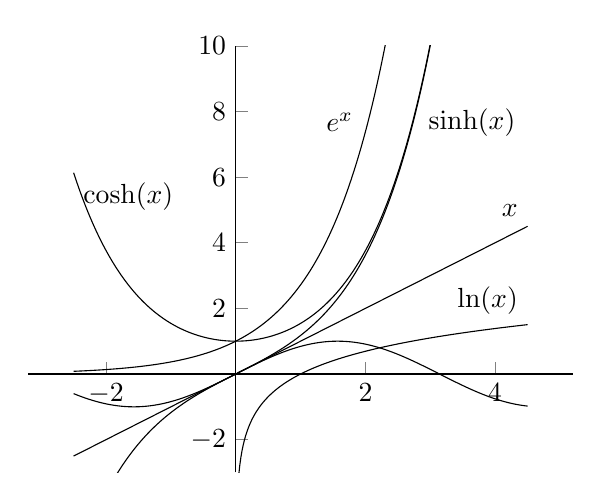
\begin{tikzpicture}
\begin{axis}[
	axis lines*=middle,
	domain=-2.5:4.5,
	samples=400,
	ymin=-3,
	ymax=10,
	height=7cm,
	width=8.5cm
]
	\addplot[mark=none]{ln(x)}    node [pos=1, above left] {$\ln(x)$};
	\addplot[mark=none]{e^x}      node [pos=0.1, above left] {$e^x$};
	\addplot[mark=none]{x}        node [pos=1, above left] {$x$};
	\addplot[mark=none]{sinh(x)}  node [pos=0.3, below right] {$\sinh(x)$};
	\addplot[mark=none]{cosh(x)}  node [pos=0, below right] {$\cosh(x)$};
	\addplot[mark=none]{sin(deg(x))};
\end{axis}
\end{tikzpicture}

\section*{Normierte und metrische Räume}

\subsection*{Normen}

\begin{description}[leftmargin=!,labelwidth=35mm]
	\item[Definitheit] $||x|| = 0 \Leftrightarrow x = 0$
	\item[Homogenität] $||\alpha x|| = |\alpha| ||x||$
	\item[Dreiecksungleichung] $||x+y|| \leq ||x|| + ||y||$
\end{description}

\subsubsection*{Konvergenz}

Folge $(x_n) \subseteq X$ konvergiert gegen $x \in X$, wenn:

$\forall \epsilon > 0 \exists N_\epsilon \in \N \forall n \geq N_\epsilon : ||x_n - x|| \leq \epsilon$

\subsubsection*{$p$-Norm}

\vspace{-4mm}
\[ |x|_p := \begin{cases}
	(\sum_{k=1}^m |x_k|^p )^{\frac{1}{p}} & 1 \leq p < \infty \\
	\max_{1\leq k \leq m} |x_k|           & p = \infty
\end{cases} \]

\subsubsection*{Hölder-Ungleichung}

Sei $p \in |1, \infty]$ mit $\frac{1}{p}+\frac{1}{p'}=1$ sowie $x, y \in \K^m$:

$|\sum_{k=1}^m x_k y_k| \leq \sum_{k=1}^m |x_k y_k| \leq |x|_p |x|_{p'}$

\subsubsection*{Minkowski-Ungleichung}

Sei $x, y \in \K^m$: $|x+y|_p \leq |x|_p + |y|_p$

\subsubsection*{Cauchy-Schwarz-Ungleichung}

Sei $(x|y) = \sum_{k=1}^m x_k \overline y_k$ Skalarprodukt, dann:

$|(x|y)| \leq \sum_{k=1}^m |x_k y_k| \leq |x|_2 |y|_2$

\subsubsection*{Kugeln}

\begin{description}[leftmargin=!,labelwidth=22mm]
	\item[offen] $B(x,r) = \{y \in X | ||x-y|| < r\}$
	\item[abgeschlossen] $\overline B(x,r) = \{y \in X | ||x-y|| \leq r\}$
	\item[Sphäre] $S(x,r) = \{y \in X | ||x-y|| = r\}$
\end{description}

\subsubsection*{Äquivalenz}

$||\cdot|| \sim |||\cdot||| \Leftrightarrow \exists C, c > 0 \forall x \in X \land r > 0 : \\ \hspace*{5mm} \overline B_{|||\cdot|||}(x, \frac{r}{C}) \subseteq B_{||\cdot||}(x, \frac{r}{C}) \subseteq B_{|||\cdot|||}(x, \frac{r}{c})$

\subsubsection*{Konvergenz bezüglich $p$-Normen}

Sei $1 \leq p < q \leq \infty$, $x \in \K^m$, dann gilt:

$|x|_p \leq m^{\frac{1}{p} - \frac{1}{q}} |x|_q$ und $|x|_q \leq |x|_p$

\subsubsection*{Cauchyfolgen bzgl. Normen}

Sei $(X, ||\cdot||)$ normierter Vektorraum. $(x_n) \subseteq X$ ist Cauchyfolge, wenn gilt:

$\forall \epsilon > 0 \exists N_\epsilon \in \N \forall n, m \geq N_\epsilon : ||x_n - x_m|| \leq \epsilon$

\subsection*{Normen stetiger Funktionen}

$C([a, b])$ ist Vektorraum mit $dim(C([a, b])) = \infty$.

Für $f \in C([a, b])$ gilt:

\begin{description}[leftmargin=!,labelwidth=15mm]
	\item[Supnorm] $||f||_\infty = \displaystyle\sup_{a\leq t \leq b} |f(t)| = \displaystyle\max_{a\leq t\leq b} |f(t)|$
	\item[1-Norm] $||f||_1 = \int_a^b |f(t)| dt$
\end{description}

\subsubsection*{Banachraum}

Wenn jede Cauchyfolge in $(X, ||\cdot||)$ einen Grenzwert besitzt, dann heißt $||\cdot||$ vollständig und $(X, ||\cdot||)$ ist Banachraum.

\subsubsection*{Hilbertraum}

Die Norm des Banachraums $(\K^m, |\cdot|_2)$ ist durch Skalarprodukt gegeben. Ein solcher Banachraum heißt Hilbertraum.

Ein $\R$-VRaum mit SKP ist ein euklidischer Raum.

\subsubsection*{Äquivalenz der Normen}

Sei $V$ endlichdim. VRaum, dann sind alle Normen auf $V$ äquivalent. Insb. ist $V$ ein Banachraum.

\subsection*{Metriken}

\begin{description}[leftmargin=!,labelwidth=35mm]
	\item[Definitheit] $d(x, y) = 0 \Leftrightarrow x = y$
	\item[Symmetrie] $d(x, y) = d(y, x)$
	\item[Dreiecksungleichung] $d(x, z) \leq d(x, y) + d(y, z)$
\end{description}

\subsubsection*{Konvergenz bzgl. Metriken}

$(x_n) \subseteq X$ konvergiert in $(M, d)$ gegen $x \in X$, wenn:

$\forall \epsilon > 0 \exists N_\epsilon \in \N \forall n \geq N_\epsilon : d(x_n, x) \leq \epsilon$

\subsubsection*{Cauchyfolgen bzgl. Metriken}

Eine Folge $(x_n) \subseteq M$ heißt Cauchfolge, wenn:

$\forall \epsilon > 0 \exists N_\epsilon \in \N \forall n, m \geq N_\epsilon : d(x_n, x_m) \leq \epsilon$

Ein metrischer Raum ist vollständig, wenn jede Cauchfolge in $(M, d)$ konvergiert.

\section*{Topologische Grundbegriffe}

Sei $M$ ein metrischer Raum, dann:

\begin{enumerate}[label=(\alph*)]
	\item $O \subseteq M$ ist offen in $M$, wenn $\forall x \in O \exists r = r(x) > 0 : B(x, r) \subseteq O$
	\item $U \subseteq M$ ist Umgebung in $M$ von $x \in M$, wenn $\exists r > 0 : B(x, r) \subseteq U$
	\item $A \subseteq M$ ist abgeschlossen in $M$, wenn $M\setminus A$ in $M$ offen ist
\end{enumerate}

\subsection*{Charakterisierung}

Sei $M$ metrischer Raum und $A, O \subseteq M$, dann gilt:

\begin{enumerate}[label=(\alph*)]
	\item $A$ ist abgeschlossen in $M$ gdw. $(x_n \in A \land \lim_{n \to \infty} x_n = x \in M ) \Rightarrow x \in A$
	\item $O$ ist offen in $M$ gdw. $\nexists x \in O : \exists y_n \in M \setminus O : \lim_{n \to \infty} y_n = x$
\end{enumerate}

$M$ und $\emptyset$ sind offen und abgeschlossen in $M$.

Die Vereinigung beliebig vieler und der Durschnitt endlich vieler offener Teilmengen von $M$ sind wieder offen in $M$.

Der Durschnitt beliebig vieler und die Vereinigung endlich vieler abgeschlossener Teilmengen von $M$ sind wieder abgeschlossen in $M$.

\subsection*{Inneres, Abschluss und Rand}

Sei $M$ metrischer Raum und $\emptyset \neq N \subseteq M$, dann ist:

\begin{description}[leftmargin=!,labelwidth=15mm]
	\item[Innere] $N^\circ = \bigcup \{ O \subseteq N | O \text{ offen in } M \}$
	\item[Abschluss] $\overline N = \bigcap\{A \subseteq M | A \text{ abg. in } M, N \subseteq A\}$
	\item[Rand] $\partial N = \overline N \setminus N^\circ = \overline N \bigcap (M \setminus N^\circ)$
\end{description}

$N^\circ$ ist die größte in $M$ offene Teilmenge von $N$.

Die Menge $N$ ist in $M$ offen gdw. $N = N^\circ$.

\vspace*{-6mm}
\begin{align*}
	N^\circ &= \{x \in M | \exists r > 0 : B(x, r) \subseteq N\} \\
	        &= \{x \in M | \nexists (x_n) \in M \setminus N : \displaystyle\lim_{n \to \infty} x_n = x\}
\end{align*}
\vspace*{-6mm}

$\overline N$ ist die kleinste in $M$ abg. Obermenge von $N$.

Die Menge $N$ ist in $M$ abgeschlossen gdw. $N = \overline N$

$\overline N = N^\circ \cup \partial N = \{x \in M | \exists x_n \in N : \lim_{n \to \infty} x_n = x \}$

$\partial N$ ist abgeschlossen in $M$.

$\partial N = \{ x \in M \\ \hspace*{8.5mm} | \exists x_n \in N, y_n \in M \setminus N : \displaystyle\lim_{n \to \infty} x_n = \displaystyle\lim_{n \to \infty} y_n = x \}$

\subsection*{Dichtheit}

$N$ dicht in $M$ $\Leftrightarrow \forall x \in M \exists (x_n) \in N : \displaystyle\lim_{n \to \infty} x_n = x$

\subsection*{Stetigkeit}

Seien $M, N$ metrische Räume, $f : M \rightarrow N$.

\subsubsection*{Gleichmäßige Stetigkeit}

$\forall \epsilon > 0 \exists \delta_\epsilon > 0 \forall x, y \in M : d_M(x, y) \leq \delta_\epsilon \Rightarrow d_N(f(x), f(y)) \leq \epsilon$

\subsubsection*{Lipschitz Stetigkeit}

$f$ ist Lipschitz stetig mit Konstante $L > 0$, wenn:

$\forall x, y \in M : d_N(f(x), f(y)) \leq L d_M(x, y)$

Lipschitz stetige Fkt. sind insb. auch glm. stetig.

$L(V, W) = \{T : V \rightarrow W | T \text{ linear} \}$ sind lineare Abb. zwischen $\K$-VR $V$ und $W$, genannt Operatoren.

\subsubsection*{Operatornorm}

Seien $V$, $W$, $Z$ endlichdim. norm. VRäume, $T \in L(V, W)$ und $S \in L(W, Z)$. Dann gelten:

\begin{enumerate}[label=(\alph*)]
	\item $T$ ist Lipschitz stetig mit Konstante \\ $||T|| = ||T||_{L(V, W)} := \sup_{x\in V \setminus \{O\}} \frac{||Tx||}{||x||}$
	\item $\forall x \in V : ||Tx|| \leq ||T|| ||x||$
	\item $||\cdot||_{L(V,W)}$ heißt Operatornorm
	\item $||ST|| \leq ||S|| ||T||$
	\item $L(V, W)$ ist Banachrm. bzgl. Operatornorm
\end{enumerate}

\subsubsection*{Banachscher Fixpunktsatz}

Sei $M$ metr. Raum und $f : M \rightarrow M$ strikte Kontraktion, d.h. $\exists q \in [0, 1) \forall x,y \in M : d(f(x), f(y)) \leq q d(x,y)$. Dann $\exists! x_* \in M : f(x_*) = x_*$

\subsection*{Kompaktheit}

Eine Teilmenge eines endlichdim. norm. Vektorraum ist nach Bolzano-Weierstraß kompakt gdw. sie beschränkt und abgeschlossen ist.

\subsubsection*{Homöomorphismus}

Seien $K$, $N$ metrische Räume, $K$ kompakt, $A \subseteq K$ abgeschlossen, $f: K \rightarrow N$ stetig. Dann gilt:

$f(A)$ ist in $N$ kompakt.

$f$ injektiv $\Rightarrow f^{-1} : f(K) \rightarrow K$ stetig

$f$ bijektiv $\Rightarrow f$ ist homömorph, d.h. bijektiv, stetig und hat stetige Umkehrabbildung.

\subsubsection*{Satz vom Maximum}

Sei $K$ komp. metr. Raum, $f: K \rightarrow \R$ stetig, dann:

$\exists x_{\pm} \in K : f(x_+) = \displaystyle\max_{x \in K} f(x) \land f(x_-) = \displaystyle\min_{x \in K} f(x)$

\subsubsection*{Wegzusammenhang}

Metr. Raum $M$ ist wegzusammenhängend gdw.:

$\forall x, y \in M \exists w \in C([0,1], M) : w(0) = x \land w(1) = y$

\subsubsection*{Zwischenwertsatz}

Sei $M$, $N$ metr. Räume, $M$ wegzusammenhängend und $f \in C(M, N)$. Dann ist $f(M)$ wegzusammenhängend. Für $N = \R$ ist $f(M)$ ein Intervall.

\section*{Differentialrechnung in VRäumen}

\subsection*{Kurventangente}

Sei $J$ ein Intervall. Ein Weg ist stetige Abbildung $f = (f_1 \hdots f_m)^T : J \rightarrow \R^m$. Das Bild $\Gamma = f(J)$ heißt Kurve. $f$ ist Parametrisierung von $\Gamma$.

Die Ableitung eines $C^1$-Wegs $f$ in $t_0 \in J$ ist def.:

$f'(t_0) = \displaystyle\lim_{h \to 0} \frac{1}{h} (f(t_0 + h) - f(t_0)) = \begin{pmatrix} f_1'(t_0) \\ \vdots \\ f_m'(t_0)\end{pmatrix} \in \R^m$

Für $f'(t_0) \neq 0$ ist Tangente $T(\R)$ an $f(t_0)$ durch $T(t) = f(t_0) + (t - t_0)f'(t_0)$ mit $t \in \R$ gegeben.

\subsection*{Partielle Ableitungen}

$\partial_j f(x) = \partial_{x_j} f(x) = \frac{\partial f}{\partial x_j}(x) := \displaystyle\lim_{t \to 0} \frac{1}{t}(f(x+te_j)-f(x))$

\subsection*{Die Ableitung}

Seien $V$, $W$ endlichdim. norm. VRäume, $D \subseteq V$ offen, $f: D \rightarrow W$, $x_0 \in D$, $r > 0$ mit $B_V(x_0, r) \subseteq D$ und betrachte $h \in V$ mit $0 < ||h||_V < r$. $f$ heißt differenzierbar in $x_0$, wenn $\exists A \in L(V, W)$ so, dass:

$\displaystyle\lim_{||h||_V \to 0} \frac{1}{||h||_V}||f(x_0 + h) - f(x_0) - Ah||_W = 0$

$f'(x_0) := A$ ist Ableitung von $f$ bei $x_0$. Wenn $\forall x_0 \in D : f $ differenzierbar, dann ist $f$ diffbar auf $D$ und $f' : D \rightarrow L(V,W)$ ist Ableitung von $f$.

\subsubsection*{Jacobimatrix}

Sei $D \subseteq \R^l$ offen, $f : D \rightarrow \R^k$, $i \in \{1, ..., k\}$, $j \in \{1, ..., l\}$ und $f = (f_1 \hdots f_m)^T$, dann:

$\partial f(x) = \begin{pmatrix} \partial_1 f_1(x) & \hdots & \partial_l f_1(x) \\ \vdots & & \vdots \\ \partial_1 f_k(x) & \hdots & \partial_l f_k(x) \end{pmatrix}$

\subsubsection*{Gradient}

Wenn $D \subseteq \R^m$ offen und $f : D \rightarrow \R$ bei $x \in D$ differenzierbar ist, dann:

$\nabla f(x) := \begin{pmatrix} \partial_1 f(x) \\ \vdots \\ \partial_m f(x) \end{pmatrix} = f'(x)^T \in \R^m$

Identifiziert kritische Stellen mit $\nabla f(x) = 0$.

\subsection*{Richtungsableitung}

Sei $D \subseteq \R^m$ offen, $f : D \rightarrow \R$ und $v \in \R^m \setminus \{0\}$, dann ist Ableitung von $f$ bei $x$ in Richtung $v$:

$\partial_v f(x) = \frac{\partial f}{\partial v}(x) := \displaystyle\lim_{t \to 0} \frac{1}{t} (f(x+tv)-f(x))$

Insofern Grenzwert in $\R$ existiert. Weiterhin gilt:

$\partial_v f(x) = (\nabla f(x) | v)$ für $f \in C^1(D, \R)$.

\subsubsection*{Hessematrix}

Wenn $D \subseteq \R^m$ offen und $f \in C^n(D, \R)$, dann $\nabla f \in C^1(D,\R^m)$ und somit:

$\nabla^2 f(x) = \begin{pmatrix} \partial_1 \partial_1 f(x) & \hdots & \partial_m \partial_1 f(x) \\ \vdots & & \vdots \\ \partial_1 \partial_m f(x) & \hdots & \partial_m \partial_m f(x) \end{pmatrix}$

	Diese Matrix ist nach dem Theorem von Schwarz, welches ebendies besagt, symmetrisch. Laplaceop. $\Delta f(x) = \partial_{11}f(x) + ... + \partial_{mm} f(x)$ ist Spur.

\subsection*{Taylor in mehreren Dimensionen}

Sei $D \subseteq \R^l$ offen, $f \in C^{n+1}(D, \R)$, $x \in D$, $r > 0$ mit $\overline B(x,r) \subseteq D$ und $h \in \R^l$ mit $|h|_2 < r$, dann:

$T_{n,x} f(x+h) = f(x) + \displaystyle\sum_{j=1}^n \frac{1}{j!} \displaystyle\sum_{\alpha_1, ..., \alpha_j=1}^l h_{\alpha_1} \cdot \hdots \cdot h_{\alpha_j} ( \partial_{\alpha_1} \hdots \partial_{\alpha_j} f )(x)$

Dies bedeutet insbesondere für $n=2$:

$f(x+h) = f(x) + (\nabla f(x)|h) + \frac{1}{2}(\nabla^2 f(x)h|h) + O(|h|_2^3)$

\subsubsection*{Restglied}

$R_{n,x} f(x+h) = f(x+h) - T_{n,x}f(x+h)$

\subsection*{Definitheit}

Sei $A \in L(\R^m)$ symmetrisch, dann ist $A$:

\begin{description}[leftmargin=!,labelwidth=28mm]
	\item[positiv definit]     $\forall v \in \R^m \setminus \{0\} : (Av|v) > 0$
	\item[negativ definit]     $\forall v \in \R^m \setminus \{0\} : (Av|v) > 0$
	\item[positiv semidefinit] $\forall v \in \R^m : (Av|v) \geq 0$
	\item[negativ semidefinit] $\forall v \in \R^m : (Av|v) \leq 0$
\end{description}

\subsubsection*{Definitheit von $2\times 2$ Hessematrizen}

Sei $A = \begin{pmatrix} a & b \\ b & d \end{pmatrix} \in \R^{2 \times 2}$ eine symmetrische Matrix:

\begin{enumerate}[label=(\alph*)]
	\item positiv definit $\Leftrightarrow$ $a > 0, ad > b^2$
	\item negativ definit $\Leftrightarrow$ $a < 0, ad > b^2$
	\item positiv semidefinit $\Leftrightarrow$ $a \geq 0, d \geq 0, ad \geq b^2$
	\item negativ semidefinit $\Leftrightarrow$ $a \leq 0, d \leq 0, ad \geq b^2$
	\item indefinit $\Leftrightarrow ad < b^2$
\end{enumerate}

\subsubsection*{Definitheit über Eigenwerte}

\begin{enumerate}[label=(\alph*)]
	\item positiv definit $\Leftrightarrow \forall \lambda \in Spec(A) : \lambda > 0$
	\item negativ definit $\Leftrightarrow \forall \lambda \in Spec(A) : \lambda < 0$
	\item positiv semidefinit $\Leftrightarrow \forall \lambda \in Spec(A) : \lambda \geq 0$
	\item negativ semidefinit $\Leftrightarrow \forall \lambda \in Spec(A) : \lambda \leq 0$
\end{enumerate}

\subsection*{Extremstellen}

Seien $D \subseteq \R^m$ offen, $f \in C^2(D, \R)$, $x \in D$, dann:

\begin{description}[leftmargin=!,labelwidth=28mm]
	\item[Maximum] $\nabla^2 f(x)$ negativ semidefinit
	\item[Minimum] $\nabla^2 f(x)$ positiv semidefinit
\end{description}

Wenn $\nabla f(x) = 0$:

\begin{description}[leftmargin=!,labelwidth=28mm]
	\item[Maximum (strikt)] $\nabla^2 f(x)$ negativ definit
	\item[Minimum (strikt)] $\nabla^2 f(x)$ positiv definit
\end{description}

\subsection*{Umkehrsatz}

Seien $D \subseteq \R^m$ offen, $f \in C^1(D, \R^m)$, $x_0 \in D$, $y_0 = f(x_0)$, $f'(x_0) \in L(\R^m$ bijektiv, dann:

$\exists U \subseteq D \text{ offen }, V \subseteq \R^m : x_0 \in U, y_0 \in V, f_U : U \rightarrow V \text{ bijektiv }, V \subseteq f(D), (f_U)^{-1} \in C^1(V, U), \forall x \in U : f'(x) \text{ invertierbar}$. Insbesondere:

$\forall y=f(x) \in V : (f_U^{-1})'(y) = f'(f_U^{-1}(y))^{-1} = f'(x)^{-1}$

\subsubsection*{Diffeomorphismen}

Seien $D \subseteq \R^m$ offen, $f \in C^1(D, \R^m)$, $\tilde D = f(D)$, $f$ injektiv, $\forall x \in D: f'(x)$ invertierbar. Dann ist $\tilde D$ offen und $f : D \rightarrow \tilde D$ ein Diffeomorphismus, d.h. $D$, $\tilde D$ offen, $f$ bijektiv und $f \in C^1(D, \R^m)$, $f^{-1} \in C^1(\tilde D, \R^m)$

\subsubsection*{Polarkoordinaten}

$\phi : D = (\R \setminus \{0\}) \times \R \rightarrow \R^2; (r, \varphi) \mapsto \begin{pmatrix} r \cos \varphi \\ r \sin \varphi \end{pmatrix} = \begin{pmatrix} x \\ y \end{pmatrix}$

\subsection*{Satz über implizit definierte Funktionen}

Seien $D \subseteq \R^{m+k}$ offen, $f \in C^1(D, \R^k)$, $(x_0, y_0) \in D$ mit $f(x_0, y_0) = 0$ und $(\partial_y f)(x_0, y_0) \in L(\R^k)$ bijektiv. Dann $\exists \text{ offene } U_x \subseteq \R^m, U_y \subseteq \R^k$ sowie Abbildung $\varphi \in C^1(U, \R^k)$ mit:

\begin{enumerate}[label=(\alph*)]
	\item $(x_0, y_0) \in U_x \times U_y \subseteq D$, $\varphi(U_x) \subseteq U_y$, $\varphi(x_0)=y_0$, $\forall (x, y) \in U_x \times U_y : \partial_y f(x,y) \in L(\R^k)$ bijektiv
	\item $(x, y) \in U_x \times U_y \land f(x,y)=0 \\ \Leftrightarrow x \in U_x \land y=\varphi(x)$
	\item $\varphi'(x) = -[(\partial_y f)(x, \varphi(x))]^{-1}(\partial_x f)(x, \varphi(x))$
\end{enumerate}

Insbesondere auch $\forall x \in U_x : f(x, \varphi(x))=0$

\subsection*{$C^1$-Flächen}

$M \subseteq \R^3$ ist eingebettete $C^1$-Fläche, wenn $\forall p \in M \exists \text{ offene } V, U \subseteq \R^3 : p \in V \land \psi : V \rightarrow U$ so, dass $\psi(V \cap M) = U \cap (\R^2 \times \{0\})$. $\psi$ heißt dann Karte.

\subsubsection*{Charakterisierung}

\begin{enumerate}[label=(\alph*)]
	\item $M$ ist $C^1$-Fläche
	\item $\forall p \in M \exists \text{ offenes } D \subseteq \R^3 \land g \in C^1(D, \R) : \\ p \in D \land \forall w \in D : \nabla g(w) \neq 0 \land M \cap D = \{w\in D | g(w) = 0\}$ (lokale Nullstellenmenge)
	\item $\forall p \in M \exists i < j \in \{1, 2, 3\}, \text{ offene } U_1 \subseteq \R^1, U_2 \subseteq \R^2, h \in C^1(U_2, U_1) : p_k \in U_1, (p_i, p_j) \in U_2$ mit $\{k\} = \{1, 2, 3\} \setminus \{j, j\}$, $h(U_2) \subseteq U_1$ und für $Z=\{x \in \R^3 | (x_i, x_j) \in U_2, x_k \in U_1\}$ gilt $M \cap Z = \{x \in \R^3 | (x_i, x_j) \in U_2, x_k = h(x_i, x_j)\}$ (lokaler Graph)
	\item $\forall p \in M \exists \text{ offenes } U_0 \subseteq \R^2, W \subseteq \R^3, F \in C^1(U_0, \R^3) : p \in W, \forall (s, t) \in U_0 : Rg(F'(s, t)) = 2$ und $F: U_0 \rightarrow M \cap W$ bijektiv mit stetiger Umkehrabbildung. (lokale Parameterisierung)
\end{enumerate}

\subsubsection*{Tangentialraum}

Tangentialraum an $m$ bei $p=F(u_0)$ wobei $F$ lokale Parametrisierung:

$T_p M = F'(u_0)(\R^2) = \left\{ F'(u_0) \begin{pmatrix} s \\ t \end{pmatrix} \middle| s, t \in \R \right\}$

\subsubsection*{Normalenraum}

Normalenraum an $M$ bei $p$ und $g(p)=0$ wobei $g$ lokale Nullstellenmenge:

$N_p M = lin\{\nabla g(p)\} = \{t\nabla g(p) | t \in \R\}$

\subsection*{Lagrange}

Seien $D \subseteq \R^l$ offen, $f \in C^1(D, \R$ und $g \in C^1(D, \R^k)$ mit $1 \leq k \leq l$. Setze $M=\{z\in D| g(z)=0\}$. $f$ besitze auf $M$ ein Extremum bei $z_0 \in M$ und $g'(z_0)$ habe Rang $k$. Dann existieren Lagrangesche Multiplikatoren $\lambda_1, ..., \lambda_k \in \R$ so, dass:

$\nabla f(z_0) = \lambda_1\nabla g_1(z_0) + \hdots + \lambda_k\nabla g_k(z_0)$

Ferner gilt $g_1(z_0) = 0, \hdots, g_k(z_0)=0$.

\section*{Kurvenintegrale}

Sei $\gamma \in C([a, b], \R^m)$ ein Weg und $\Gamma = \gamma([a, b])$ die dazugehörige Kurve. Die Länge von $\Gamma$ wird durch Polygonzüge approximiert. Sei dazu $a \leq b$ und $\mathcal{Z}(a, b)$ die Menge aller Zerlegungen $Z = \{a = t_0, t_1, ..., t_{n-1}, t_n = b\}$. Für $Z \in \mathcal{Z}$ wird gesetzt:

$l(\gamma, Z) = \sum_{j=1}^n |\gamma(t_j) - \gamma(t_{j-1})|_2$

\subsection*{Rektifizierbarkeit}

$\gamma : [a, b] \rightarrow \R^m$ ist rektifizierbar, wenn:

$l_{[a, b]}(\gamma) = ||\gamma||_{BV} := \sup_{Z\in \mathcal{Z}} l(\gamma, Z) < \infty$

$l(\gamma)$ ist dann die Länge von $\gamma$.

\subsubsection*{Wegintegral}

Sei $\gamma \in C^1([a, b], \R^m)$, dann ist $\gamma$ rektifizierbar mit:

$l(\gamma) = \int_a^b |\gamma'(t)|_2 dt$

\subsection*{Kurvenintegrale und Potentiale}

Sei $\gamma \in C([a, b], \R^m)$ stückweise $C^1$, $\Gamma = \gamma([a, b])$.

\subsubsection*{Kurvenintegral erster Art}

Sei reelles $f \in C(\Gamma, \R)$ gegeben:

\vspace*{-5mm}
\[ \int_\Gamma f d\gamma = \int_\Gamma f(x) d\gamma := \int_a^b f(\gamma(t)) | \gamma'(t) |_2 dt \]

\subsubsection*{Kurvenintegral zweiter Art}

Sei vektorwertiges $F \in C(\Gamma, \R^m)$ gegeben:

\vspace*{-5mm}
\[ \int_\Gamma F \cdot dx = \int_\Gamma F(x) \cdot dx := \int_a^b (F(\gamma(t))|\gamma'(t)) dt \]

\subsubsection*{Wegunabhängigkeit}

Sei $D \subseteq \R^m$ offen, dann ist $F \in C(D, \R^m)$ wegunabhängig auf $D$, wenn für alle stückweisen $C^1$-Kurven $\gamma_1, \gamma_2 \in C([a, b], \R^m)$ in $D$ mit gleichem Anfangs- und Endpunkt gilt:

\[ \int_{\Gamma_1} F \cdot dx = \int_{\Gamma_2} F \cdot dx \]

Ein $\phi \in C^1(D, \R)$ heißt Potential von $F$ auf $D$, wenn $\nabla\phi = F$ auf $D$. $F$ ist dann Gradientenfeld.

Weiterhin ist $F$ wegunabhängig auf $D$ gdw. $F$ ein Potential $\phi$ auf $D$ hat.

Ferner gilt dann: $\int_\Gamma F \cdot dx = \phi(\gamma(b))-\phi(\gamma(a))$

\subsubsection*{Poincar\'e}

Sei $D \subseteq \R^m$ offen und sternförmig und $F \in C^1(D, \R^m)$ sei rektifizierbar. Dann hat $F$ ein Potential auf $D$, insbesondere auch auf jeder Kugel $B(x_0, r) \subseteq D$.

\section*{Gewöhnliche Differentialgleichung}

\subsection*{Lokale Lipschitzstetigkeit}

Sei $M \subseteq \R^m$ und $J$ ein Intervall. $g : J \times M \rightarrow \R^k$ ist lokal Lipschitz in $x$, wenn:

$\forall (t_0, x_0) \in J \times M \exists \delta = \delta(t_0, x_0) > 0, r = r(t_0, x_0) > 0, L = L(t_0, x_0) \geq 0 \forall t \in [t_0 - \delta, t_0 + \delta] \cap J \forall x, y \in \overline B(x_0, r) \cap M : |g(t,x) - g(t, y)|_2 \leq L|x-y|_2$.

$f$ Lipschitz $\Rightarrow f$ lokal Lipschitz $\Rightarrow f$ stetig.

$f$ stetig differenzierbar $\Rightarrow f$ lokal Lipschitz.

Ein diff. $f$ ist Lipschitz gdw. $\partial_x^{(1)} f$ beschränkt ist.

\subsection*{Anfangswertprobleme}

Seien $J \subseteq \R$ ein Intervall, $t_0 \in J$ mit $t_0 < \sup J$, $D \subseteq \R^m$ offen, $f \in C(J \times D, \R^m)$ und $u_0 \in D$.

\vspace*{-4mm}
\begin{align*}
	u'(t)  &= f(t, u(t)), t\geq t_0, t\in J \\
	u(t_0) &= u_0
\end{align*}

Für das Anfangswertproblem wird ein $t_1 \in J$ mit $t_1 > t_0$ und eine eindeutige Lösung $u \in C^1([t_0, t_1], \R^m)$ auf $[t_0, t_1]$ gesucht.

\subsubsection*{Lokale Lipschitzstetigkeit im Kontext}

Sei $f \in C(J \times D, \R^k)$, $D \subseteq \R^m$ offen, $J$ ein Intervall und es existieren alle partiellen Ableitungen $\frac{\partial}{\partial x_j} f \in C(J \times D, \R^k)$ für $j \in \{1, \hdots, m\}$.

Dann ist $f$ lokal Lipschitz in $x$.

\subsubsection*{Picard-Lindelöf (lokal)}

Seien $J$ ein Intervall, $D \subseteq \R^m$ offen, $f \in C(J \times D, \R^m)$ lokal Lipschitz in $x$, $u_0 \in D$, $t_0 \in J$ mit $t_0 < \sup J$. Dann gelten:

\begin{enumerate}[label=(\alph*)]
	\item $\exists t_1 = t_1(u_0) > t_0 $ mit $t_1 \in J$ und eine eindeutige Lösung $u$  auf $[t_0, t_1]$ von $u'(t) = f(t, u(t))$ mit $u(t_0) = u_0$
	\item $u'(t) = f(t, u(t))$ mit $u(t_0) = u_0$ besitze zwei Lösungen $v_1$ und $v_2$ auf Intervallen $[t_0, T_1] \subseteq J$ bzw. $[t_0, T_2] \subseteq J$. Dann stimmen $v_1$ und $v_2$ auf $[t_0, T_3]$ mit $T_3 = \min\{T_1, T_2\}$ überein.
\end{enumerate}

\subsubsection*{Picard-Lindelöf (maximal)}

Unter den Voraussetzungen von Picard-Lindelöf (lokal) sei $u_0 \in D$, dann gilt weiterhin:

\begin{enumerate}[label=(\alph*)]
	\item $\exists$ maximale Existenzzeit $\overline t(u_0) \in (t_0, \sup J]$ und eine eindeutige maximale Lösung $u$ von $u'(t) = f(t, u(t))$ mit $u(t_0) = u_0$ auf $[t_0, \overline t(u_0))$
	\item Wenn $\overline t(u_0) < \sup J$, dann $\exists t_n \in (t_0, \overline t(u_0))$ mit $\lim_{n \to \infty} t_n = \overline t(u_0)$ so, dass die Blow-Up Bedingung erfüllt ist: $\lim_{n \to \infty} |u(t_n)|_n = \infty$ oder $\lim_{n \to \infty} \inf_{x \in \partial D} |u(t_n) - x|_2 = 0$
\end{enumerate}

\subsubsection*{Gronwallsche Ungleichung}

Sei $J$ ein Intervall, $\varphi \in C(J)$, $\varphi \geq 0$, $t_0 = \min J$ und $a, b \geq 0$ Konstanten mit $\forall t \in J : 0 \leq \varphi(t) \leq a+b \int_{t_0}^t \varphi(s) ds$. Dann gilt: $\forall t \in J : \varphi(t) \leq a e^{b(t-t_0)}$

\subsubsection*{Obergrenze des Existenzintervall}

Seien $J = [t_0, \infty)$, $D \subseteq \R^m$ offen, $M \subseteq \R^m$ abgeschlossen mit $M \subseteq D$, $f \in C(J \times D, \R^m)$ sei lokal Lipschitz in $x$, $u$ die maximale Lösung von $u'(t) = f(t, u(t))$ auf $[t_0, t(u_0))$ und es gelte $\forall t_0 \leq t \leq \overline t(u_0) : u(t) \in M$. Dann gelten:

\begin{enumerate}[label=(\alph*)]
	\item $\forall b > t_0 \exists c(b) \geq 0 : \forall t \in [t_0, b], x \in M : (f(t,x)|x) \leq c(b) (1+|x|_2^2) \Rightarrow \overline t(u_0) = \infty$
	\item Sei speziell $f: D \rightarrow \R^n$ und $\exists c \geq 0$ mit $\forall x \in M : (f(x)|x) \leq c(1+|x|_2)$, dann $\overline t(u_0) = \infty$
\end{enumerate}

Bedingung (a) folgt aus: $\forall b > t_0 \exists \tilde c(b) \geq 0 \\ \hspace*{4mm} \forall t \in [t_0, b], x \in M : |f(t,x)|_2 \leq \tilde c(b)(1+|x|_2)$

Bedingung (b) folgt aus: $\exists \tilde c > 0 \forall x \in M : \\ \hspace*{4mm} |f(x)|_2 \leq \tilde c(1+|x|_2)$

\subsubsection*{Formulierung als Problem 1. Ordnung}

Jedes Anfangswertproblem $k$-ter Ordnung lässt sich in ein Problem 1. Ordnung umschreiben.

Beispielsweise: Das Problem 2. Ordnung $u''(t)=h(t)-u(t)+u'(t)^2$ mit $u(0)=u_0$ und $u'(0)=u_1$ sowie $h \in C(\R, \R)$ wird formuliert als Problem 1. Ordnung:

\[ \begin{pmatrix}u(t)\\u'(t)\end{pmatrix}' = \begin{pmatrix}u'(t)\\u''(t)=h(t)-u(t)+u'(t)^2\end{pmatrix} \]

Sei $v_0(t):=u(t)$, $v_1(t):=u'(t)$ und $v(t):=\begin{pmatrix}v_0(t)\\v_1(t)\end{pmatrix}$

\vspace*{-4mm}
\begin{align*}
	g : \R^3 &\rightarrow \R^2 \\
	\begin{pmatrix}t\\v_0\\v_1\end{pmatrix} &\mapsto \begin{pmatrix}v_1\\h(t)-v_0+v_1^2\end{pmatrix}
\end{align*}

Insgesamt also:

\vspace*{-4mm}
\begin{align*}
	v'(t)&=g(t,v(t))=\begin{pmatrix}v_1(t)\\h(t)-v_0(t)+v_1(t)^2\end{pmatrix}\\
	v(0)&=\begin{pmatrix}u_0\\u_1\end{pmatrix}
\end{align*}

\subsubsection*{Trennung der Variablen}

Sei $u'(t)=g(t)h(u(t))$ mit $u(t_0)=u_0$ Anfangswertproblem mit $g \in C(\R, \R)$, $h \in C((a, b), \R)$, $u_0 \in (a, b)$ und $h(u_0) \neq 0$. $u$ ist Lösung, wenn $J$ Intervall mit $\forall t \in J : u(t) \in (a, b)$, $u \in C^1(J, \R)$ und $t_0 \in J$.

\vspace*{-5mm}
\[ u \text{ ist Lösung } \Rightarrow \int_{t_0}^t g(s) ds = \int_{u_0}^{u(t)} \frac{1}{h(x)} dx \]
\vspace*{-3mm}

Dies kann manchmal nach $u$ aufgelöst werden.
